% useful commands to delete build files : 
% rm *.aux *.log *.out *.fdb_latexmk *.gz *.fls 


\documentclass{article}
\usepackage[scaled]{helvet}
\renewcommand{\familydefault}{\sfdefault} % applies font
\usepackage{tcolorbox}

\usepackage[left=0.3in, right=0.6in, top=0.05in, bottom=0.5in]{geometry}
\usepackage{graphicx}
\usepackage{hyperref}
\usepackage{enumitem}
\usepackage{fancyhdr}
\usepackage{titlesec}
\usepackage{microtype}
\usepackage{xcolor} % Required for text color

% Define your own custom commands, styles, or formatting here

\pagestyle{fancy}
\fancyhf{}
\rhead{Alfred LALANNE}
\lhead{Dossier de compétences}
\cfoot{\thepage}

\title{Dossier de compétences}
\author{Alfred LALANNE}
\date{} % Remove the date

% Redefine \maketitle to remove the date and include photo
\makeatletter
\renewcommand{\maketitle}{%
    \begin{center} % Center the whole content
        \centering
        
        {\Large\bfseries \@title \par}
        \vskip 0.5em%
        {\large \@author \par}
        \begin{minipage}[b]{0.6\linewidth} % left minipage
            
        \end{minipage}%
        \hfill % Add some horizontal space between the minipages
        \begin{minipage}[b]{0.3\linewidth}   % right minipage
            \raggedleft
            \vspace*{-2\baselineskip} % Adjust the vertical position of the title
            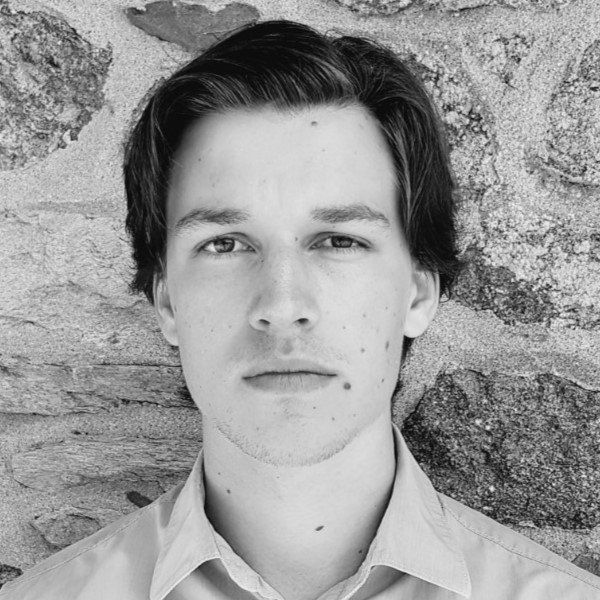
\includegraphics[width=0.7\linewidth]{moi.jpeg}
        \end{minipage}%
    \end{center} % End of center environment
}
\makeatother




\begin{document}

\maketitle

%\section{Domaines de compétence}

\begin{flushright}
    \begin{minipage}[t]{0.1\textwidth} % Left minipage
        \textbf{Domaines de compétences}
 
    \end{minipage}%
    \hspace{0.05\textwidth} % Space between minipages
    \begin{minipage}[t]{0.8\textwidth} % Right minipage
        \begin{itemize}[label={}, leftmargin=*, topsep=0pt, partopsep=0pt, itemsep=0pt, parsep=0pt] % Remove bullet points and adjust left margin
            \setlength{\itemsep}{0pt} % Reduce spacing between lines
            \item Hardware - Electronique 
            \begin{itemize}[label={--}, leftmargin=*, topsep=0pt, partopsep=0pt, itemsep=0pt, parsep=0pt] % reduce spacing & adjust left margin
                \item \textcolor{gray!80}{Transistors : polarisation, technologie, logique }
                \item \textcolor{gray!80}{Schémas électriques, routage }
                \item \textcolor{gray!80}{Filtrage analogique actif et passif, Matlab}
            \end{itemize}
            \item Electronique numérique 
            \begin{itemize}[label={--}, leftmargin=*, topsep=0pt, partopsep=0pt, itemsep=0pt, parsep=0pt] % reduce spacing & adjust left margin
                \item \textcolor{gray!80}{Microcontrôleurs : programmation en C et Assembleur sur Keil-uVision }
                \item \textcolor{gray!80}{Logique programmable : technologie FPGA, description VHDL}
                \item \textcolor{gray!80}{Systèmes sur puce : SoC, SoC-FPGA, SoC-IP}
            \end{itemize}
            \item Informatique 
            \begin{itemize}[label={--}, leftmargin=*, topsep=0pt, partopsep=0pt, itemsep=0pt, parsep=0pt] % reduce spacing & adjust left margin
                \item \textcolor{gray!80}{Langages : C, C++, Python, Java, Assembleur}
                \item \textcolor{gray!80}{Environnements : x86, ARM, VMs Linux, compilation croisée, FreeRTOS, microcontrôleurs}
                \item \textcolor{gray!80}{IDE : STM32CubeIDE, VSCode, Eclipse}
                \item \textcolor{gray!80}{Outils collaboratifs : Git, Jira, Confluence, Teams}
            \end{itemize}
            \item Ingénierie système
            \begin{itemize}[label={--}, leftmargin=*, topsep=0pt, partopsep=0pt, itemsep=0pt, parsep=0pt] % reduce spacing & adjust left margin
                \item \textcolor{gray!80}{Rédaction de cahier des charges}
                \item \textcolor{gray!80}{Etudes de faisabilité}
            \end{itemize}
        \end{itemize}
    \end{minipage}
\end{flushright}

\section{Experience}
% Your work experience details go here

\section{Projects}
% Details of your projects go here

\section{Skills}
% List of your skills goes here

\section{Achievements}
% Any awards or achievements you want to showcase

\section{References}
% References or contacts for further information

\end{document}